\documentclass[10pt,conference,compsocconf]{IEEEtran}

\usepackage{hyperref}
\usepackage{graphicx}	% For figure environment
\usepackage{amssymb} % for checkmarks

\begin{document}
\title{SELFIES or SMILES? A case study in chemical reaction prediction.}

\author{
  Matthias Kellner, Tim Kircher\\
  \textit{Machine Learning CS-433 : Project 2, EPFL}
}

\maketitle

\begin{abstract}
    Chemical reaction prediction is a key process of the drug development pipeline in medicinal chemistry. Accurate prediction of reaction products given a set of reactants is one important aspect of chemical reaction modelling. Recent work on reaction prediction is focused on neural machine translation with Simplified Molecular-Input Line-Entry System (SMILES) molecular representations. SMILES representations are not robust and a large fraction of randomly generated SMILES do not correspond to valid molecules. Due to this, a robust string-based molecular representation Self-referencing Embedded Strings (SELFIES) has been developed. This work explores the comparison of SMILES and SELFIES molecular representations in the context of chemical reaction prediction with transformer models.
\end{abstract}

\section{Introduction}

The abstraction of complex physico-chemical processes into rules and simple notations is a key instrument in the toolbox of any chemist. Common examples include skeletal visualisation of organic molecules and representation of reactions mechanisms by electron movement with arrows. Generally, these notations are useful for understanding chemical processes based on a set of heuristic rules. String based representations of molecular graphs can describe these heuristics.An example for skeletal chemical formulae, corresponding string representations and the reaction prediction workflow are displayed in figure \ref{fig:chemical_prediction_example}
Recently machine learning methods have been explored for chemical reaction prediction.\cite{ReactionPredictionReview,MolecularTransformer} Performing chemical reaction prediction in a supervised machine-learning setting with neural networks necessitates both a suitable model architecture and representation of chemical information. 


\subsection{Computational Chemical Reaction Prediction}

Chemical reaction prediction describes mapping input molecules to output molecules\cite{ReactionPredictionReview}. Predicting the main product from a reaction mixture is the most simple task, where the input are the reactants and the output is the main product. Computational reaction prediction methods may be divided into template- and template-free methods\cite{MolecularTransformer,SELFIES}. Template methods rely on handcrafted expert rules, while template-free methods do not require domain knowledge. In a big data setting template-free methods are preferable because they are scalable. Template-free methods are further divided into graph-based methods and seq2seq methods. Graph-based methods utilise atom-mapping and map the location of an atom in the reactants, described by adjacency matrices, to the location of the atom in the products. seq2seq modelling utilises methods from neural machine translation to map the reactant string to the product string. 

\begin{figure}[t!]
    \centering
    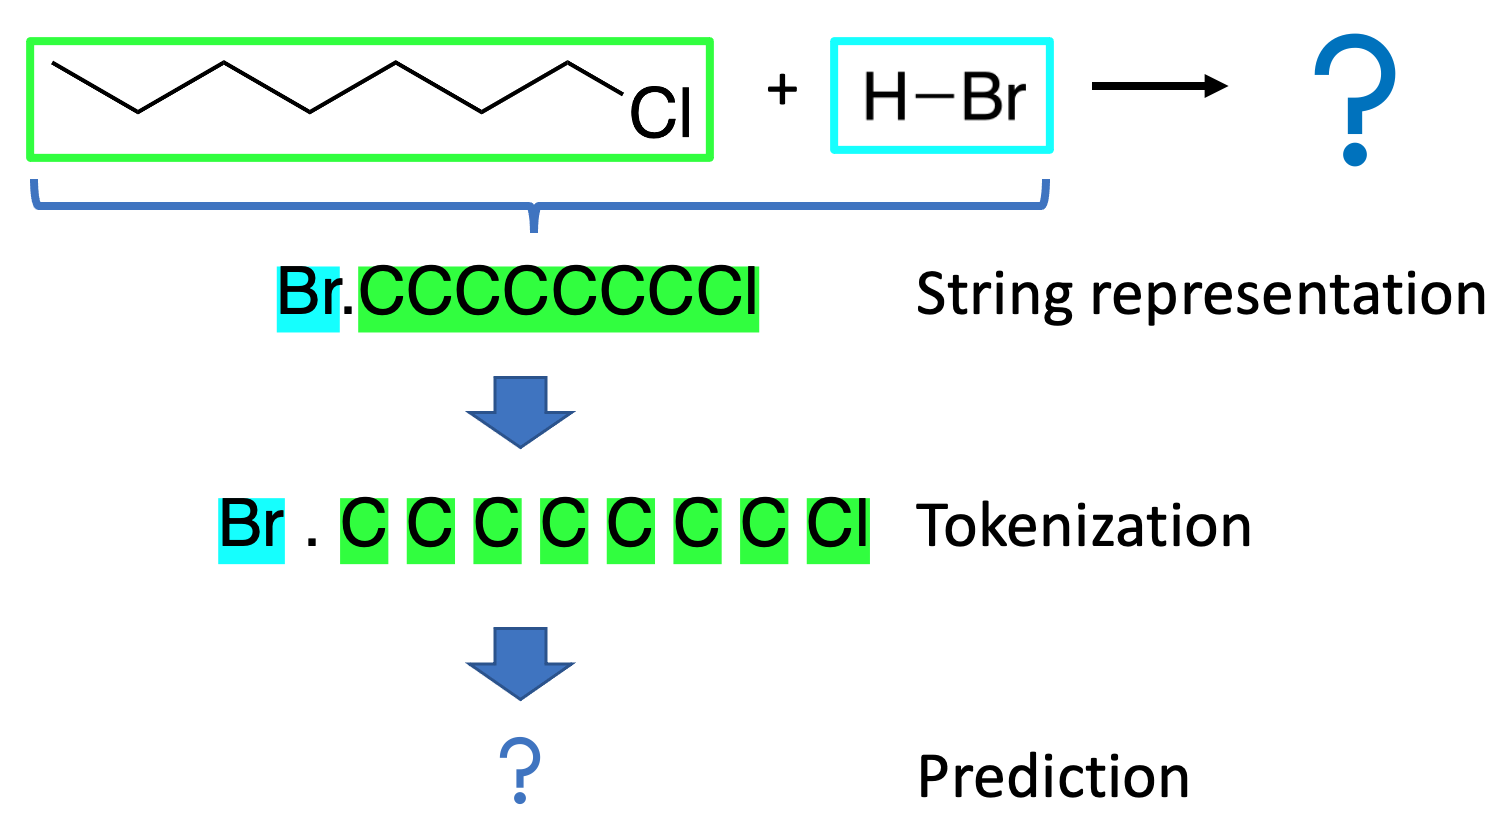
\includegraphics[width = .9\linewidth]{./figures/reaction_prediction.png}
    \caption{Reaction prediction workflow from skeletal formula of 1-chloroheptane with hydrobromic acid, corresponding string representation, tokenization and product prediction. }
    \label{fig:chemical_prediction_example}
\end{figure} 

\subsection{String-Based Molecular Representations}

Application of seq2seq modelling to chemical problems requires a memory efficient machine-readable representation of chemical information. SMILES is the most common string based molecular representation and is widely used in computational chemistry.\cite{MolecularTransformer} SMILES is based on graph theory and molecular information is embedded into letters and symbols by a simple set of rules\cite{Weininger1988SMILESAC,Weininger1989SMILES2A}. Critically, the representation power of SMILES in not restricted to chemically feasible molecules.\cite{SELFIES} It is therefore possible for a SMILES to correspond to a non-valid molecule. This poses a significant design flaw for generative models. SELFIES are an alternative, robust string-based molecular representation.\cite{SELFIES} Representation rules for SELFIES are derived from a systematically derived formal grammar. Each SELFIE string, even randomly generated SELFIE strings, corresponds to a valid molecule. Figure \ref{fig:encoding} shows the canonical SMILES and the corresponding SELFIE representation of 3,4-methylenedioxymethamphetamine. \\

\begin{figure*}
    \centering
    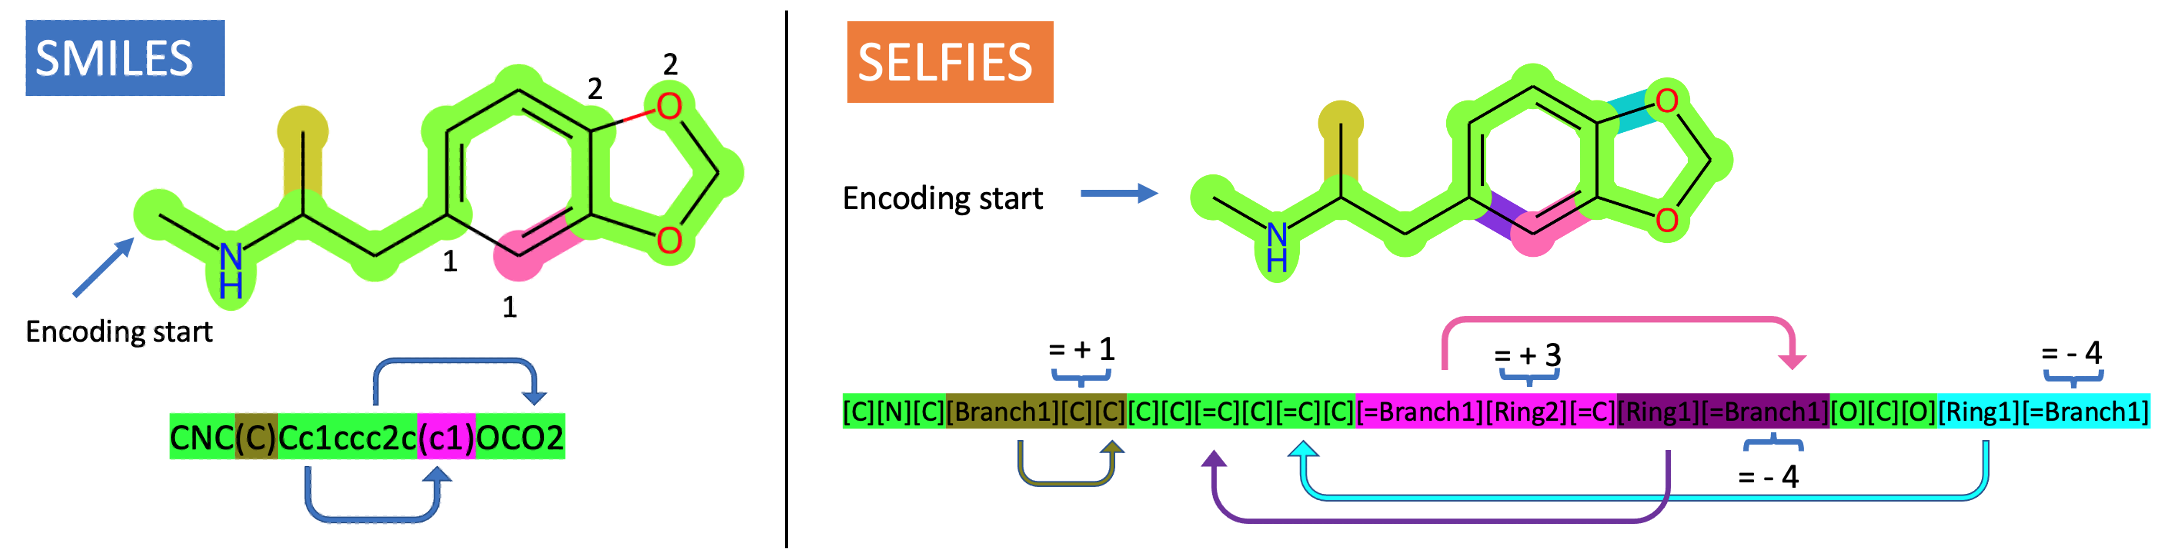
\includegraphics[width = .9\textwidth]{figures/SELFIES_SMILES_explanation.png}
    \caption{Canonical SMILES and corresponding SELFIES encoding of 3,4-methylenedioxymethamphetamine.}
    \label{fig:encoding}
\end{figure*} 

SELFIES were developed for inverse molecular design valid chemical structures are important\cite{SELFIES,SelfiesBlog}. Additionally, SELFIES have shown promising results in neural machine translation of IUPAC structures to molecular representations\cite{Selfies4NMT} and image recognition tasks of skeletal molecular formulae\cite{Selfies4ImageRecognition}. seq2seq reaction prediction is an important application of molecular representations to chemical modelling. To the best of our knowledge there exists no work on the comparison of molecular representation for seq2seq reaction prediction. This work compares molecular representations for the seq2seq modelling based on neural machine translation with transformer models.

%eine abbildung die eine reaktion zeigt und dann die selfies und smiles notation dazu


%ideas:
%main literature: 
% https://pubs.acs.org/doi/10.1021/acscentsci.9b00576 :molecular transformer
% https://iopscience.iop.org/article/10.1088/2632-2153/aba947 :selfies
%https://arxiv.org/pdf/2112.03041.pdf selfies vs smiles

%other interesting literture:
%https://jcheminf.biomedcentral.com/articles/10.1186/s13321-020-00469-w, selfies better for machine understanding?
%https://chemrxiv.org/engage/chemrxiv/article-details/60c75681567dfe722dec64d6, selfies better for machine understanding?
%https://aspuru.substack.com/p/molecular-graph-representations-and selfies blogpost

\section{Data}

We used the USPTO-480k chemical reactions dataset in this work. It is derived from patent mining by Lowe et. al \cite{lowe_extraction_2012}\cite{jin_predicting_2017} and used as a benchmark set in the research community. The reactions are described by SMILES and are separated into products and reactants. The data set contains a total of 480,000 reactions. The data set is split into a train, validation and test set containing 410000, 30000 and 40000 reactions. The data is publicly available at \url{https://github.com/coleygroup/Graph2SMILES}. The data is tokenized according to the tokenizer available at \url{https://github.com/pschwllr/MolecularTransformer}. SELFIES are generated from SMILES and tokenized by the SELFIES package \url{https://github.com/aspuru-guzik-group/selfies}. SMILES Molecules are canonicalized and checked for validity by RDKit. The conversion of canonicalized from SMILES to SELFIES and back to SMILES yielded different strings before and after the conversion for molecules containing hypervalent atoms such as phosphorous or transition metals. To circumvent this problem and ensure a closed loop for conversion between SELFIES and SMILES, hyper-valencies are allowed for SELFIES strings.\\

Two SELFIES tokenization and different data augmentation approaches are explored. For the baseline model SELFIES are tokenized according to Krenn et. al\cite{SELFIES}. Separating connected tokens, such as [Branch1] or [Ring1] is explored in SELFIES 2. Further tokenization of all SELFIES tokens is performed in SELIFES 3. Both additional tokenization approaches try to decrease the information content per SELFIES token. For data augmentation, a training set containing SMILES reactants and SELFIES products and vice-versa are explored, where SMILES and SELFIES molecular representations are seperated by "$\vert$" and the representations do not share any tokens. Finally, a training set containing both SMILES and SELFIES representations of each reactant and product are investigated. Figure \ref{fig:tokenization_approaches} shows an example for the tokenization of N-methylbutan-2-amine.

\begin{figure}[h]
    \centering
    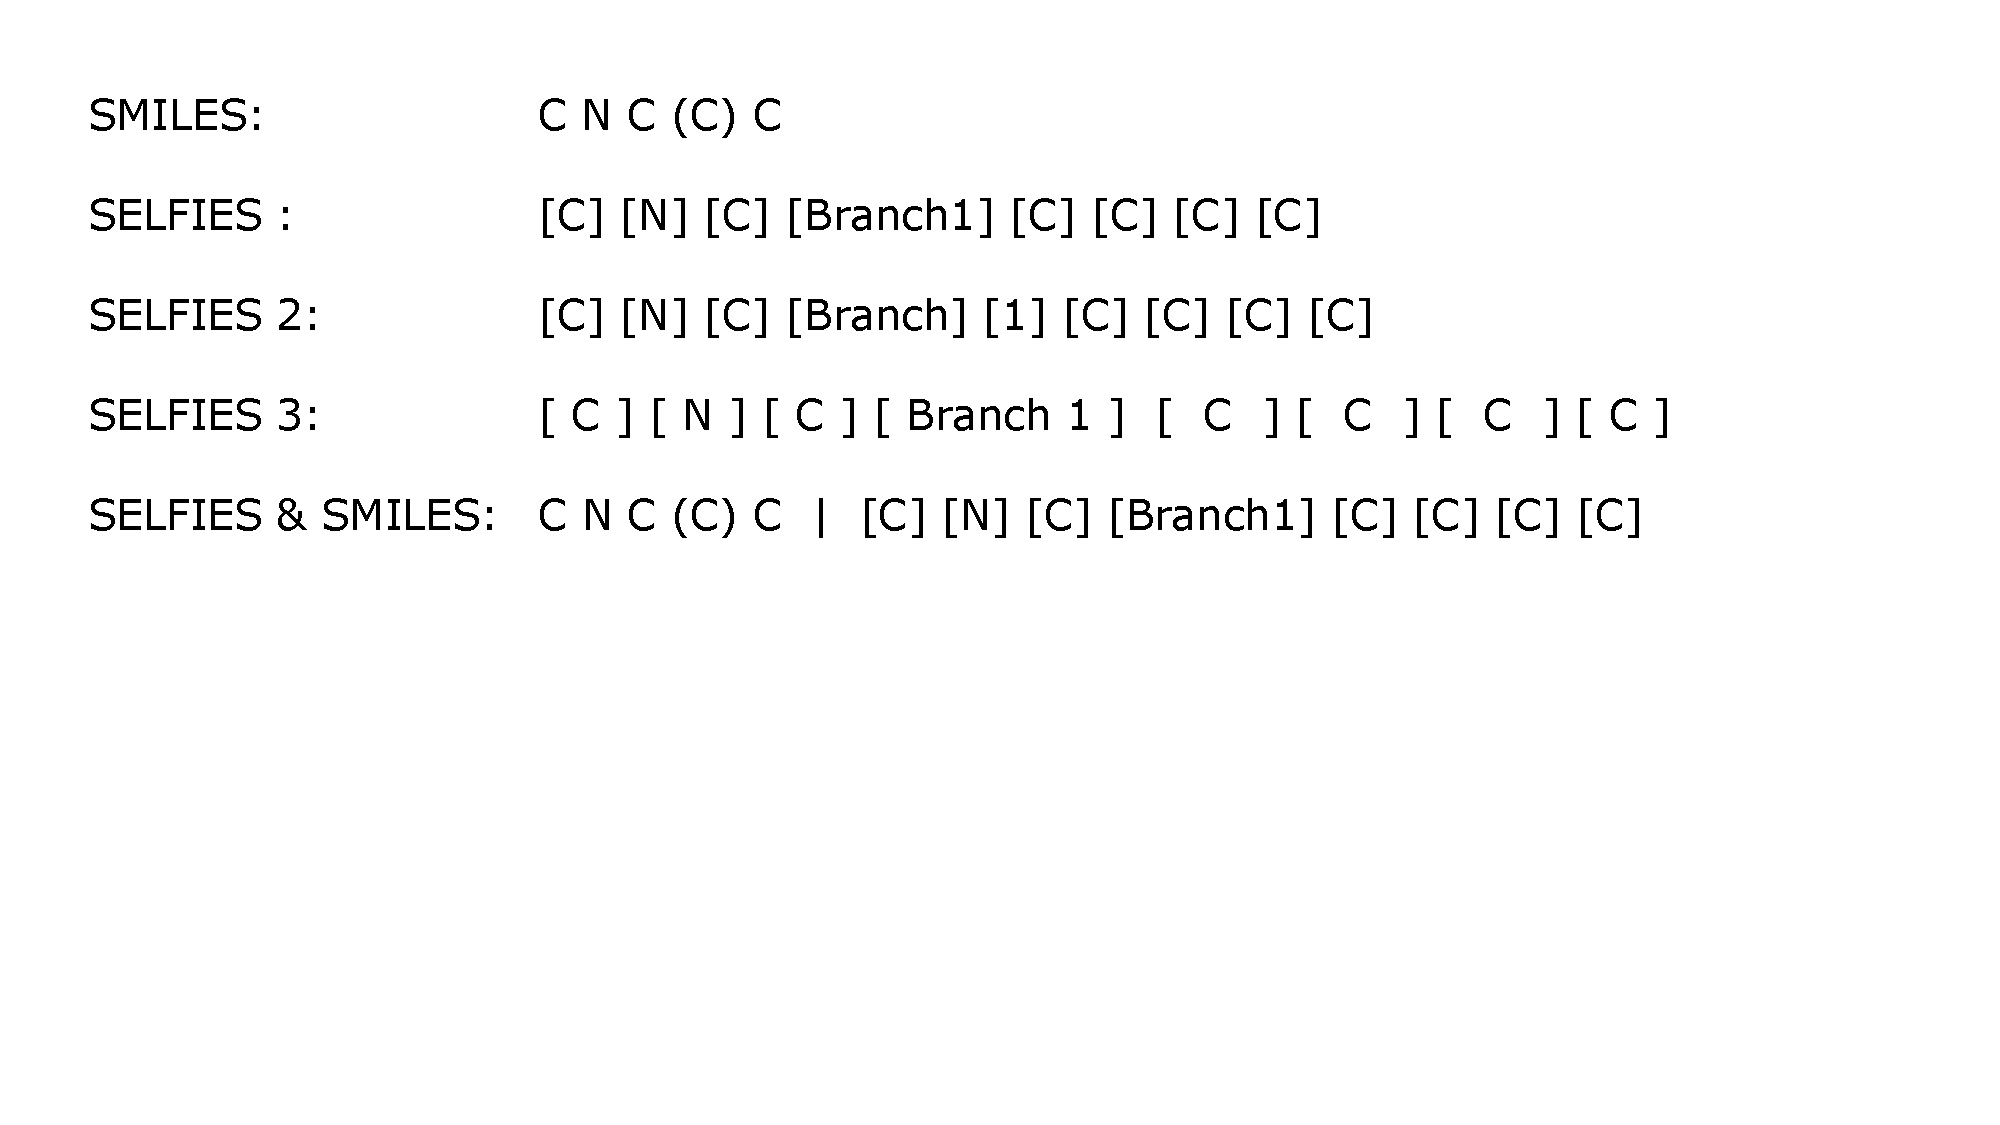
\includegraphics[width = 1\linewidth, trim={1.25cm 9.75cm 3.5cm 1.25cm},clip]{./figures/representation.pdf}
    \caption{Tokenization approaches exemplified for N-methylbutan-2-amine.}
    \label{fig:tokenization_approaches}
\end{figure} 

\section{Computational Methods}

The data and reaction predictions were handeled and analysed with the RDkit \cite{noauthor_rdkit_nodate} cheminformatics toolkit and the RDkit compatible SELFIES code (available on github).\cite{noauthor_selfies_2021}

The model used in this work is based on the carbohydrate transformer by Schwaller et. al \cite{Pesciullesi.2020}. The transformer architecture is implemented with the OpenNMT-py framework \cite{klein-etal-2017-opennmt}. Hyperparameters are taken from \url{https://github.com/rxn4chemistry/OpenNMT-py/tree/carbohydrate_transformer}. The transformer utilises an autoregressive encoder-decoder architecture with multiheaded attention and positional feed forward layers. The model has 4 hidden layers with 2048 neurons and 8 attention heads. For training the ADAM optimizer is utilised with 8000 warm-up steps. The models are trained for 250000 steps. A dropout of 0.1 and gradient normalisation over 4 batches are utilised for regularisation. In contrast to the original NMT model, label smoothening is set to 0. Models are evaluated by predicting reaction products by beam search with a beam-width of 5. Due to long model training time ($>$24~h~per~model), limited computational resources and the limited time frame of the semester project hyperparameter optimisation is not explored and the identical set of hyperparameters is utilised for all models.

\section{Results}
We trained the transformer model on the USPTO-480K reaction data set. The resulting Top-1 and Top-5 validation set accuracies on SMILES and SELFIES using different tokenization and data augmentation approaches are evaluated. Top 1 accuracy denotes the model accuracy when predicting a single product and Top 5 accuracy denotes the number of correct predictions when 5 possible reaction products are predicted by beam search. For augmented SELFIES \& SMILES the SMILES and SELFIES the output is a string containing a predicted SELFIES and a predicted SMILES string separated by "$|$". The SELFIES and SMILES string are evaluated separately (augmented SMILES and augmented SELIFES). The molecular transformer\cite{MolecularTransformer}, trained and validated on the identical data set, is included as a benchmark. \\
\begin{table}[h!]
  \centering
  \begin{tabular}[c]{|l|l|l|}
    \hline
    Molecular Representation & Top 1 accuracy [\%] & Top 5 accuracy [\%] \\
    \hline
    SMILES & 86.0 & 92.3 \\
    SELFIES & 75.8 & 86.1 \\
    SELFIES 2 & 73.3 &  83.9 \\
    SELFIES 3 & 68.8 & 80.2 \\
    Augmented SMILES & 83.8 & 89.4 \\
    Augmented SELFIES & 74.9 & 86.2\\ \hline
    Molecular Transformer \cite{MolecularTransformer} &  88.8 & 94.4 \\
    \hline
  \end{tabular}
  \caption{Results for tokenization and data augmentation approaches on the validation set.}
  \label{tab:firstresults}
\end{table}

Table \ref{tab:firstresults} shows that SMILES molecular representation has the highest validation accuracy of the analysed molecular representations. SELFIES top-1 accuracy is significantly lower by 10~\%. Further SELFIES tokenization approaches did not yield an increased accuracy. Furthermore, data set augmentation did not increase accuracy. The accuracy for both SELFIES and SMILES with the augmented data set is slightly lower than without the augmented data set. The model is not able to transfer context of SELFIES to SMILES or vice-versa. All models are inferior to the benchmark transformer model. This is attributed to the lack of hyperparameter optimisation and lower training time in this work. The best performing SMILES model has a test accuracy of 86.4~\%.\\

SELFIES and SMILES models are further analysed to investigate the difference in model performance. Figure \ref{fig:top1} shows the Top-1 model accuracy and model steps. It also shows the progression towards the final accuracy over the first 125,000 steps. Figure \ref{fig:top1} shows that the SMILES model converges significantly faster than the SELFIES model. Also, it shows that both models are converged after 250,000 steps, as the model accuracy does not increase after 125,000 steps. Both models reach their final accuracy after 125,000 steps. Next, the prediction for SMILES and SELFIES model for each reaction in the validation set is compared. Figure \ref{fig:Venn} shows a venn diagram for shared true products, products only identified in the SMILES model and products only identified in the SELFIES model.\\
\begin{figure}[h]
    \centering
    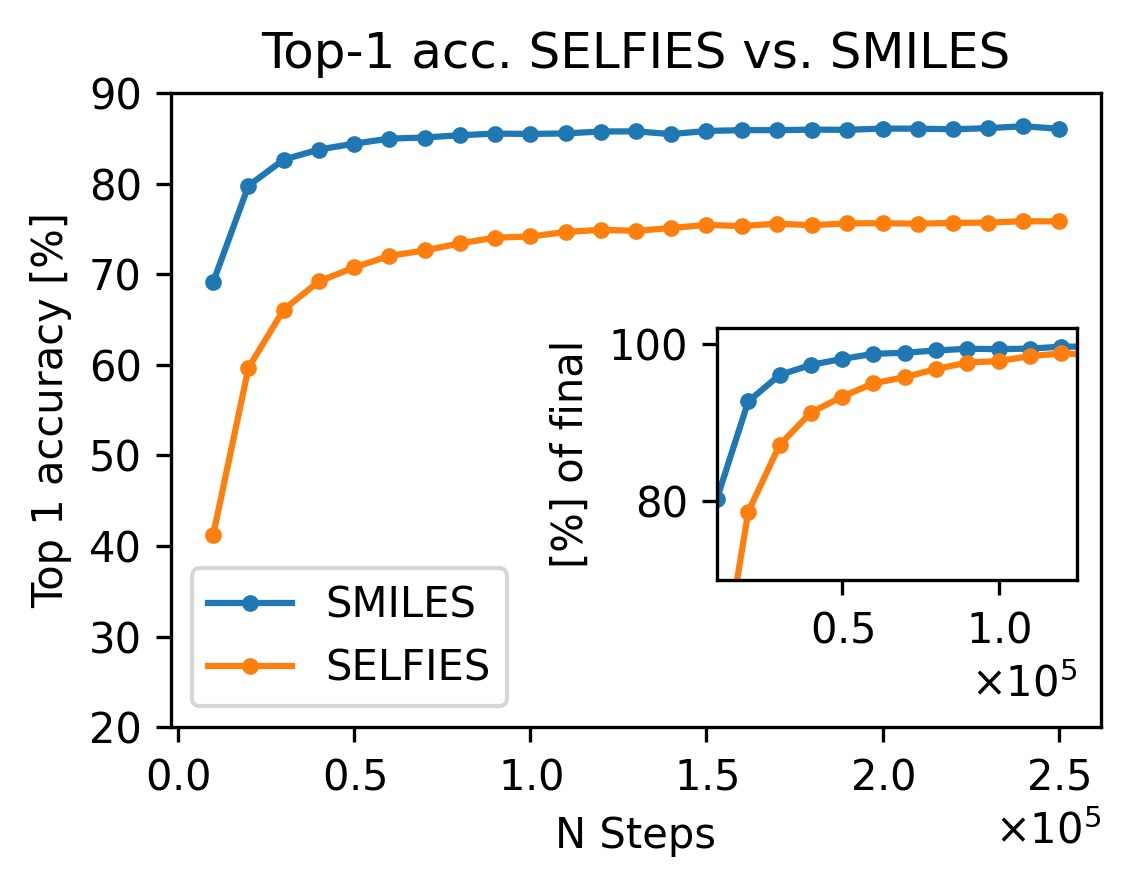
\includegraphics[width = .8\linewidth]{figures/accuracy.jpeg}
    \caption{Top-1 Validation Accuracy for SELFIES and SMILES Model.}
    \label{fig:top1}
\end{figure} 

\begin{figure}[h]
    \centering
    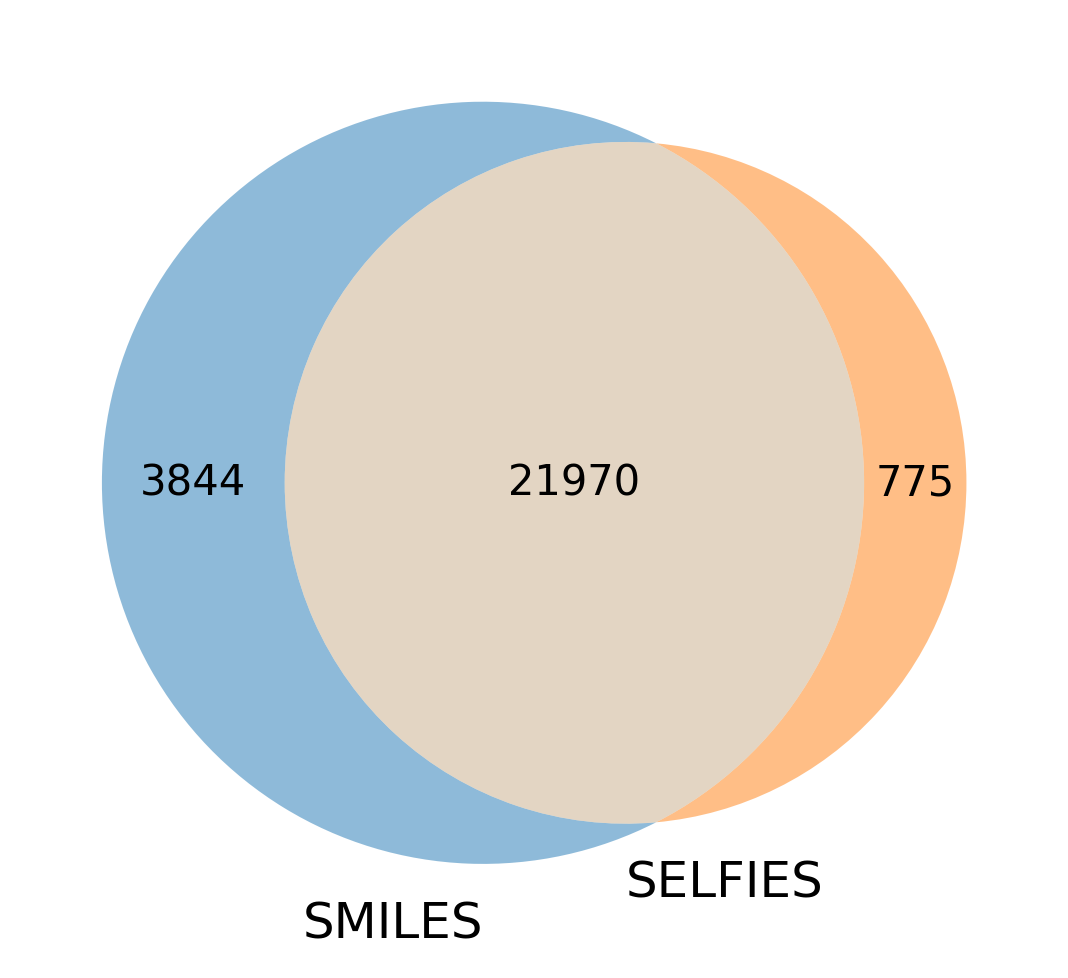
\includegraphics[width = .7\linewidth]{./figures/venn.png}
    \caption{Correctly identified products for both models, only SMILES and only SELFIES model.}
    \label{fig:Venn}
\end{figure} 

Figure \ref{fig:Venn} shows that the models for both molecular representations share a large number of correct predictions. Additionally, the SMILES model is able to predict a significant number of reactions correctly for which the SELFIES prediction is false. The number of reactions which the SELFIES model exclusively predicts correctly is far lower. This leads to the question if the difference in prediction quality is related to the chemical reaction space or the string representation encoding.\\

To address the first question of the relation between model proficiency and the chemical reaction space, the validation set is mapped in a tree plot\cite{schwaller2020mapping}. Figure \ref{fig:tree} (Appendix) shows a tree plot of the validation set. Similar reactions are are clustered and the color of a reaction data point denotes if the reaction is predicted correctly in no model, in both models, only in the SMILES model and only in the SELFIES model. Generally, 73~\% of all reactions are predicted correctly by both SELFIES and SMILES model and thus the majority of the plot is green. For the case of reactions predicted only by SELFIES or only by SMILES, no clusters may be identified. Reactions that are exclusively predicted by one of the two models share no common characteristics in the chemical space.\\

Next, the number of chemically valid products are investigated. SELFIES are a robust molecular representation and excel in generative tasks because all SELFIES strings correspond to valid molecules. Table \ref{tab:validity} shows number of chemically valid molecules predicted by the SELFIES and SMILES model. Invalid molecules are detected by RDKit utilising the DetectChemistryProblems function. SELFIES are converted to SMILES to check for validity.

\begin{table}[h]
  \centering
  \begin{tabular}[c]{|l|l|l|}
    \hline
    Molecular Representation & Valid Molecules [\%] \\
    \hline
    SMILES & 99.3 \\
    SELFIES & 98.3 \\
    \hline
  \end{tabular}
  \caption{Percentage of chemically valid molecules predicted by the model on the validation set according to valency rules.}
  \label{tab:validity}
\end{table}

Surprisingly, not all SELFIES correspond to valid molecules. The proportion of chemically invalid molecules is higher for SELFIES than for SMILES. We attribute this to the hyper-valency settings. When hypervalencies are not allowed during the translation of predicted SELFIES to SMILES, 99.99\% of predicted molecules follow standard valency rules. For the case of the SMILES model, 0.7\% of the predicted products are invalid. Chemical validity is a main advantage of the SELFIE representation. If hypervalent atoms are present in the data set, interchangeability between SELFIES and SMILES is not possible without allowing for hyper-valency. Unfortunately this impairs the advantage of the robust SELFIES representation.\\

Exploration of the chemical space shows that reaction chemistry and model proficiency are not strongly related. We believe the prediction quality for SELFIES is impaired by token ambiguity. SELFIES tokens are ambiguous and either encode an atom or a position, depending on the context. Tokens following "[Branch]" or "[Ring]" indicate the size of the respective element. "[Branch]" and "[Ring]" tokens include a number, for example "[Branch1]", which denotes the number of following tokens used for indexing. An example for ambiguity is the "[C]" token, the most frequent token in the training set, which indicates the index 0 or a carbon atom. The string "[Branch1]~[C]~[C]" references a branch of size 1 with 1 carbon atom. Figure \ref{fig:SELFIESbad} shows the identical molecule as figure \ref{fig:encoding} on the left. The string representations of \ref{fig:encoding} and \ref{fig:SELFIESbad} differ slightly, as a different encoding start position is chosen to exemplify SELFIES ambiguity.\footnotemark On the right, a carbon atom is exchanged for a phoshine group.\\

\begin{figure}[h!]
  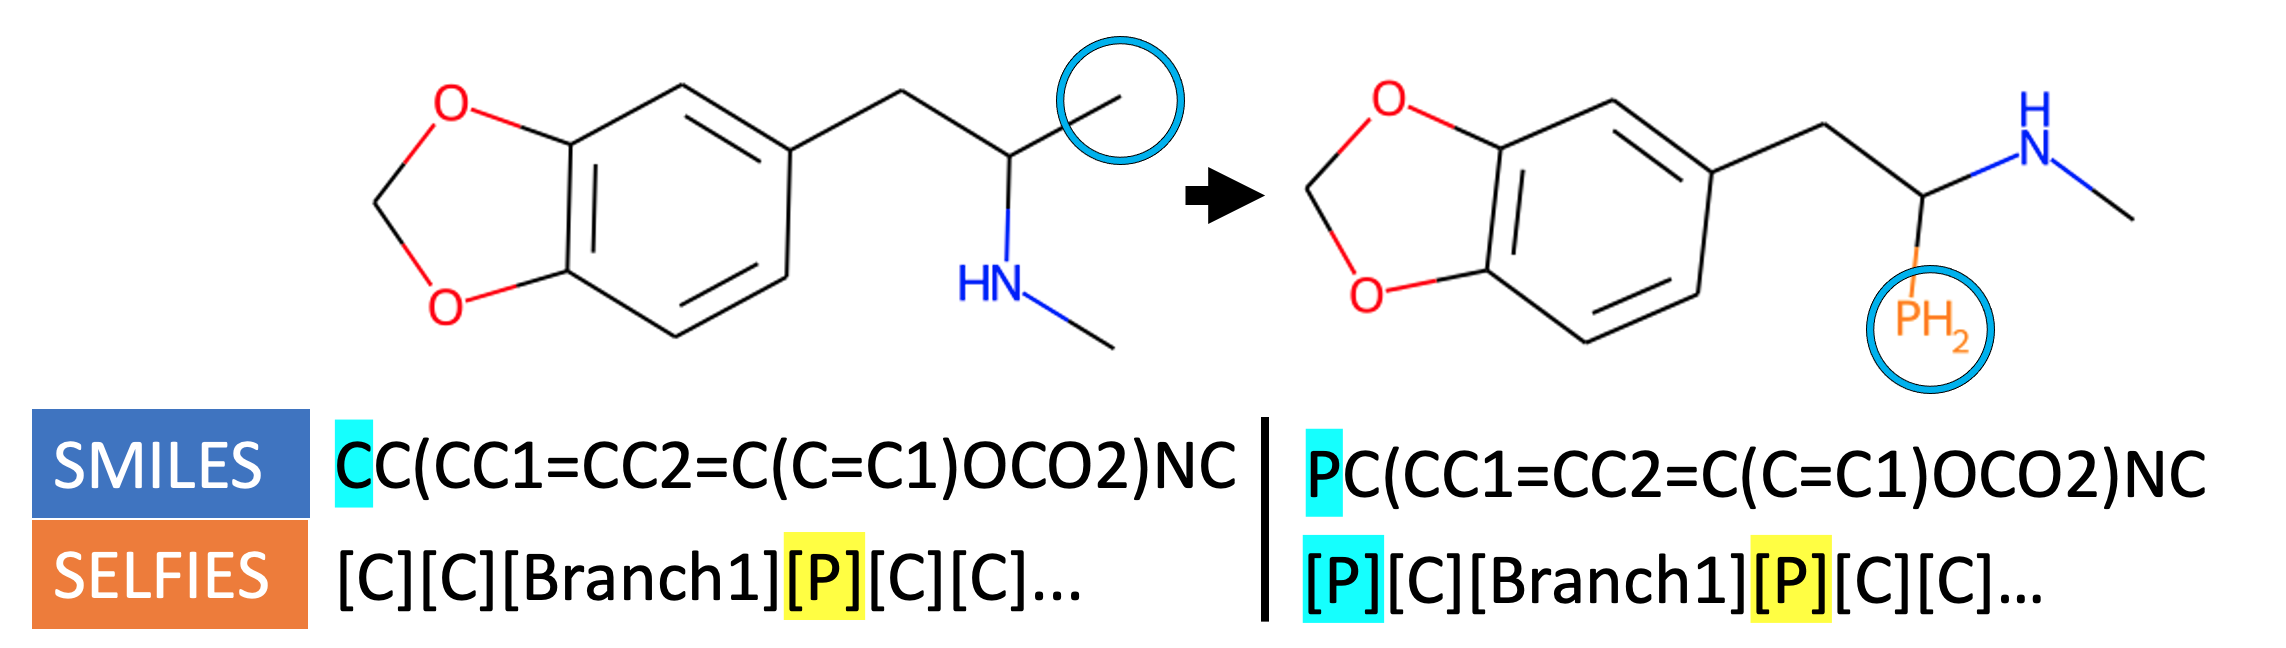
\includegraphics[width=0.45\textwidth]{figures/encode_C_P.png}
  \caption[]{Illustration the ambiguity of SELFIES}
  \label{fig:SELFIESbad}
\end{figure}
\footnotetext{When using string based molecular graph descriptors, the encoding start can be freely chosen, resulting in varying strings depending on the encoding start. Cheminformatics toolkits such as the RDkit have algorithms implemented that can transform all of the possible representation strings of one molecular graph into one unique, so called canonical string. The different SMILES encoding position has been chosen to illustrate the ambiguity of the [P] SELFIES token, after transforming the aforementioned non canonical SMILES.}

The SELFIES representation on the left includes a "[Branch1]" token followed by a "[P]" token representing a branch of 4 tokens. After introducing a phosphine group, the SELFIES string on the right contains two "[P]" with vastly different meanings. The SMILES string contains no ambiguity regarding atoms and positions. The inferior performance of SELFIES when compared to SMILES for transformer applications is mirrored by similar work, where SMILES and SELFIES are compared for chemical image recognition.\cite{Rajan2021}.

\section{Summary \& Outlook}

In this work, we find that the SELFIES molecular graph representation is outperformed by the more established SMILES representation in reaction prediction using transformer models.\\

Further analysis of the prediction outcomes shows no correlation between prediction accuracy and selected reaction types for both representations. Conclusively reaction prediction models using SMILES and SELFIES predictions share a majority of correctly predicted reactions. We attribute the slower convergence and lower prediction accuracy of the SELFIES model to the ambiguous encoding of ring- and branch closing connections in SELFIES strings. Albeit necessary for generative tasks, such as discovery of novel molecular scaffolds, this ambiguity most likely can not be captured by the transformer model. Such token ambiguity also hinders the study of the influence of locality of information in string-based molecular descriptors. So far we have not made use of the opportunities that SELFIES offer through the mutation of chemical structures exploited in generative applications. In further work, ambiguous tokens could be replaced by tokens that are not part of the SELFIES grammar, as the validity of the SELFIES after point mutation does not have to be ensured in prediction applications.

%A combined approach of structure generation and reaction prediction could be envisaged, where reaction educts are systematically varied and generated and investigated for their synthetic feasibility or possible  "reachability" through chemical reactions.
%are optimized - every combination should create a valid molecule. Is against heuristics, where only some can be stable...
%model struggles to learn structure property relationship?
%Operator overloading is nescessary to ensure that molecules are valid after point mutation

\newpage
\bibliographystyle{IEEEtran}
\bibliography{literature}

\section{Appendix}
\begin{figure*}[t]
    \centering
    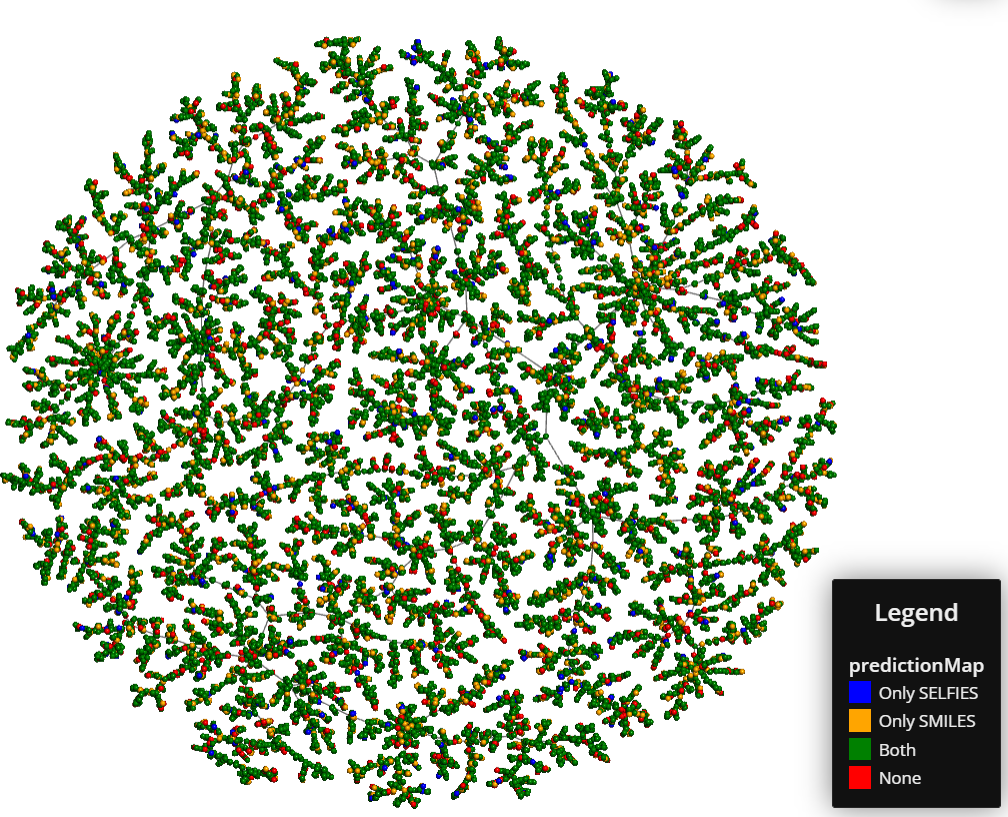
\includegraphics[width = .9\textwidth]{./figures/tree.png}
    \caption{Correctly identified reactants for both models, only SMILES and only SELFIES model and none grouped by product similarity.}
    \label{fig:tree}
\end{figure*} 

\end{document}
